\chapter{Rydberg state excitations induced by intense near-infrared radiation} % (fold)
\label{cha:rydberg_state_excitations}

In the previous chapter, we have studied ionization of atoms involving few photons. We will now turn our attention to processes in strong-field physics where many-photon processes driven by intense IR lasers are studied. When large numbers of photons are absorbed, the discrete nature of the multi-photon picture begins to blurs, allowing for processes to be understood in a complementary way through classical trajectory analysis and tunneling processes. 
Fundamental processes in strong-field atomic physics are above-threshold ionization (ATI) \cite{agostini1979}, high harmonic generation (HHG) \cite{franken1961,mcpherson1987,ferray1988}, and non-sequential double ionization \cite{walker1994}. These highly nonlinear processes are induced by the absorption of multiple photons from the laser field, which in the limit of a large photon number can also be described as a tunneling process. Excitation of the atom is known to play an important role in each of the processes. It has been initially observed via resonant enhancement in the population of excited states \cite{deboer1992,jones1992} and structures in the energy spectrum \cite{freeman1987,perry1989,agostini1989} and in energy-resolved angular distributions \cite{rottke1994} of photoelectrons. These resonance effects have been explained by multiphoton absorption through Rydberg states, which are AC-Stark shifted in the presence of a laser field. More recently, significant excitation of atoms has also been observed in the tunneling regime and described by the frustrated tunneling ionization model \cite{nubbemeyer2008}. 

For linearly polarized lasers, the latter observation has renewed the general interest in the mechanisms leading to the population of excited (Rydberg) states during the interaction of an atom with an intense laser pulse (most recently, e.g., in Refs. \cite{chini2014,li2014,li2014b,zimmermann2015,shao2015,camp2015,li2015,fechner2015,bredtmann2016,fushitani2016,lv2016,serebryannikov2016,hart2016,li2016,xiong2016,beaulieu2016,larimian2016,zimmermann2017,bengtsson2017,gao2017,ivanov2017,ilchen2017,mancuso2017,xiong2017,piraux2017}). The important role of Rydberg states in various strong-field ionization processes and harmonic generation has been discussed. For example, resonant enhancement of below-threshold harmonics \cite{toma1999,chini2014,camp2015}, emission from excited states via free induction decay \cite{camp2015,beaulieu2016}, high harmonic emission through ionization from excited states and recombination to the ground state \cite{bian2010,beaulieu2016} have been predicted and observed.

Recent theoretical studies of the excitation mechanism in linearly polarized strong fields mainly consider the distribution of the population as a function of the principal quantum number of the excited states \cite{li2014,li2014b,zimmermann2017,xiong2017,piraux2017}. It was shown that the modulation of the excitation probability is related to the channel closing effect \cite{krajewska2012,li2014,li2014b,piraux2017}. 
%The latter phenomenon occurs at threshold intensities at which the absorption of one more photon is needed to ionize the atom due to the shift of the ionization threshold by the ponderomotive energy. The interpretation that an increase in excitation can be understood as result of the shift of the first ATI peak below the ionization threshold \cite{li2014,li2014b} is in agreement with the explanation of earlier experimental results (e.g., \cite{freeman1987,jones1992,rottke1994}) via the resonance enhanced population of AC-Stark shifted excited states. 
Theoretical analysis of the angular momentum distribution in the populated Rydberg states by linearly polarized fields is less advanced. Predictions of Floquet theory for a monochromatic laser field \cite{krajewska2012} and results of numerical calculations for laser pulses with a trapezoidal envelope \cite{piraux2017} yield that the angular momentum of the excited Rydberg states has the same parity as $N_p-1$, where $N_p$ is the minimum number of photons needed to ionize the atom. Furthermore, the angular quantum number of the states with the largest population in numerical calculations \cite{li2014,li2014b,piraux2017} agrees well with semiclassical estimations \cite{arbo2008}, initially performed for low-energy angular resolved photoelectron distributions.

Besides interactions with linear polarized laser pulses, recently studies on the interaction of atoms and molecules with intense fields generated by the superposition of two circularly polarized laser pulses have seen an upsurge in activity in strong-field experiment and theory. For the most part, the renewed interest results from the capability to control the polarization of emitted light in high-order harmonic generation with such pulses. The physical principle has been proposed and applied first two decades ago 
\cite{eichmann1995,long1995}. 
More recently, efficient phase matching of circularly polarized high-order harmonic beams in the EUV and soft X-ray regime using bichromatic beams with counter-rotating circular polarization has been demonstrated \cite{fleischer2014,pisanty2014,kfir2015,fan2015,hickstein2015}. Since then, much experimental and theoretical work on high-harmonic generation \cite{milosevic2015a,medisauskas2015,milosevic2015b,chen2016,baykusheva2016,hernandez2016,liu2016,mauger2016,bandrauk2016,reich2016b,odzak2016,dorney2017,fleischer2017,zhavoronkov2017,pisanty2017,baykusheva2017,lerner2017,ayuso2018,dixit2018,barreau2018,huang2018,jimenez2018,heslar2018,paufler2018,li2019}, 
ionization and photoelectron momentum distributions
\cite{ngoko2015,yuan2016,milosevic2016c,mancuso2016,milosevic2016b,mancuso2017,pengel2017,busuladzic2017,hoang2017,lin2017,abusamha2018,busuladzic2018,eckart2018,li2018,han2018,eckart2018b,liu2018,eicke2019,ge2019,kerbstadt2019,abusamha2019}, double ionization 
\cite{mancuso2016b,eckart2016,ben2017,ngoko2017,yu2018,huang2018b,ma2019}
and other strong-field processes \cite{yuan2015,buica2018,guo2019} driven by bichromatic circularly polarized laser pulses has been performed. One interesting aspect in these kind of strong-field interactions is the control of ionization via the helicity of the applied bichromatic pulses \cite{milosevic2016c,mancuso2016,liu2018}. Such studies complement related work on the dependence of the ionization rate by one-color circularly pulse on the relative helicity between the pulse and the electron in the atomic orbital
\cite{barth2011,kazansky2012,herath2012,barth2013,bauer2014,barth2014,ooi2014,hartung2016,douguet2016,watzel2016,wang2017,zhang2017,eckart2018c,liu2018b,trabert2018}.

For the interaction with bichromatic circularly polarized laser pulses resonant excitation also plays an important role. It has been observed that the probability to ionize an atom is significantly enhanced if the two fields are counter-rotating as compared to co-rotating fields \cite{mancuso2016}. The experimental observations were interpreted as due to the increased density of excited states accessible for resonant enhanced multiphoton ionization in the case counter-rotating fields. Results of numerical solutions of the time-dependent Schr\"odinger equation in Ref.\ \cite{mancuso2016} did confirm a close relation between the ratios of total excitation and ionization probabilities for counter-rotating and co-rotating circularly polarized laser pulses. However, the results for excitation of the atom were not further resolved by distributions over the quantum numbers (principal, angular momentum, magnetic). Such analysis potentially can shed further light on the role of excited states in the pathways to ionization since excitation in a resonant multiphoton process should rely on the spin-angular momentum selection rules for the absorption of circularly polarized photons ($\Delta l = \pm 1$ and $\Delta m = \pm 1$).

%More generally, analysis of the role of strong-field excitation has recently experienced a renaissance 
%\cite{nubbemeyer2008,eichmann2013,chini2014,zimmermann2015} 
%following earlier work 
%\cite{freeman1987,perry1989,agostini1989}.
% Concerning the distribution in the excited states with respect to the quantum numbers studies for the interaction of atoms with linearly polarized pulses have been performed only. Theoretical studies have considered the distribution of the population as a function of the principal and/or the angular momentum quantum number \cite{krajewska2012,li2014,li2014b,xiong2017,piraux2017,venzke2018_ryd}. In applications of Floquet theory for a monochromatic laser field \cite{krajewska2012} and numerical calculations for laser pulses with  trapezoidal \cite{piraux2017} and Gaussian or $\sin$-squared envelopes \cite{venzke2018_ryd} it has been analyzed how the parity of the populated angular momentum states in such pulses relates to the selection rules for linearly polarized pulses. In view of the recent experimental observations discussed above, we extend these studies to interaction of atoms with bichromatic circularly polarized laser pulses. Such study provides the interesting opportunity to not only resolve the excited state distribution with respect to the principal or angular orbital momentum quantum number, but in particular to consider the role of the magnetic quantum number as well. For our studies we make use of results of numerical solutions of the time-dependent Schr\"odinger equation (TDSE) for the interaction of the hydrogen atom with intense bichromatic circularly polarized laser pulses.

In this chapter, we present results for excitation of atoms with linearly polarized (Sec.~\ref{sec:linear_polarization}) and bi-circular (Sec.~\ref{sec:bi_circular_polarization}) laser pulses. Interpretation of the distributions of excitation over the states with different quantum numbers will be given using multiphoton selection rules. 
%to predict the parity of the angular momentum quantum number of the populated excited states (Sec.~\ref{sec:linear_polarization}). Then we discus excitation induced by bi-circular IR laser pulses and interpret the results in the multiphoton picture (Sec.~\ref{sec:bi_circular_polarization}). 



%%%%%%%%%%%%%%%%%%%%%%%%%%%%%%%%%%%%%%%%%%%%%%%%%%%%%%%%%%%%%%%%%%%%%%%%%%%%%%%%%%%%%%%%%%%%%%%%%%%%%%%%%%%%%%%%%%
%%%%%%%%%%%%%%%%%%%%%%%%%%%%%%%%%%%%%%%%%%%%%%%%%%%%%%%%%%%%%%%%%%%%%%%%%%%%%%%%%%%%%%%%%%%%%%%%%%%%%%%%%%%%%%%%%%
%%%%%%%%%%%%%%%%%%%%%%%%%%%%%%%%%%%%%%%%%%%%%%%%%%%%%%%%%%%%%%%%%%%%%%%%%%%%%%%%%%%%%%%%%%%%%%%%%%%%%%%%%%%%%%%%%%
%%%%%%%%%%%%%%%%%%%%%%%%%%%%%%%%%%%%%%%%%%%%%%%%%%%%%%%%%%%%%%%%%%%%%%%%%%%%%%%%%%%%%%%%%%%%%%%%%%%%%%%%%%%%%%%%%%
%%%%%%%%%%%%%%%%%%%%%%%%%%%%%%%%%%%%%%%%%%%%%%%%%%%%%%%%%%%%%%%%%%%%%%%%%%%%%%%%%%%%%%%%%%%%%%%%%%%%%%%%%%%%%%%%%%
\section[Linear polarization]{Linear polarization\protect\footnote{The content of this section has been also published in J. Venzke et al., Physical Review A \textbf{98}, 043434 (2018).}} % (fold)
\label{sec:linear_polarization}

As mentioned before, for the interaction with linear polarization earlier work for monochromatic laser fields \cite{krajewska2012} and laser pulses with a trapezoidal envelope \cite{piraux2017} have been performed. Here, we extend these previous analysis by considering excitation in laser pulses with more realistic sine-squared and Gaussian envelopes. This gives us the opportunity to study if the parity of the populated angular momentum states in such pulses agrees with the selection rules obtained for monochromatic fields and how the results depend on the pulse length at low and high intensities. In Sec.~\ref{sub:radiation} we then investigate how the population of angular momentum states leaves its footprints in the radiation generated via transitions from the excited states to the ground state. 

For our studies we have made use of results of numerical solutions of the time-dependent Schr\"odinger equation (TDSE) for the interaction of the hydrogen atom with an intense linearly polarized laser pulse.
% The paper is organized as follows: In Sec.\ \ref{sec:theory} we briefly discuss theoretical aspects of the excitation process in strong fields as well as the numerical methods used for the solutions of the time-dependent Schr\"odinger equation. In Sec.\ \ref{sec:angularmomentum} we present numerical results for angular momentum distributions in resonantly excited states. In particular, we focus on the effects of intensity and pulse length on the distribution. Finally, in Sec.\ \ref{sec:radiation}, numerical results for the high harmonic generation spectra are presented and analyzed in view of signatures of the population in the excited states. We summarize our results in Sec.\ \ref{sec:summary}. We use Hartree atomic units, $e = m = \hbar = 1$, throughout the article unless stated otherwise.
Specifically, we are solving the time-dependent Schr\"{o}dinger equation (TDSE) for the interaction of an atom with a linearly polarized intense laser pulse in the velocity gauge (Eq.~\ref{eq:SAE}) for the Hydrogen atom ($V_{SAE}(r)=-1/r$). The code utilizes cylindrical coordinates and second order finite difference. In all calculations presented below we used a grid ranging up to $\rho=$ 750 a.u. and $z=$ $\pm$750 a.u. with a grid spacing of $\Delta =$ 0.1 a.u. in both directions and a time step of $\Delta t = 0.15$ a.u. We use the outer 37.5 a.u. of the grid in both directions for the ECS potential. This grid can easily fit bound states up to $n = 14$ within the real portion of the grid. 

\subsection{Angular momentum distributions}
\label{sub:angularmomentum}

\subsubsection{Parity effect in pulses}
\label{ssub:parity}
We study the angular momentum distribution in Rydberg states of the hydrogen atom. To this end, we consider processes during which these states are shifted into resonance with multiphoton absorption from the initial ground state of the atom (with energy $E_i$). Assuming that the energy shift of high lying excited states under the influence of an intense laser field is approximately equal to the ponderomotive shift \cite{agostini1989} and the shift occurs instantaneously during the pulse \cite{he2011}, the intensity for a $N_p$ photon process to resonantly excite  approximately with an excited state with energy $E_n$ is then given by:
%
\begin{equation}
I = 4\omega_E^2(N_p\omega_E + E_i - E_n).
\end{equation}
%
In our calculations we have considered peak intensities such that the $n=8$ states are in resonance at central frequency $\omega_E$, corresponding to a wavelength of 800 nm, with $N_p = 10, 11, \ldots, 15$ photon processes. Since we study the interaction with laser pulses, instead of monochromatic fields, more than one manifold of states can be resonantly excited. For example, the bandwidth of a 20 cycle sine squared pulse at 800 nm covers all excited states $n \gtrapprox 6$ within the same $N_p$ photon process. We further note that in the present cases, the $n=3$ and $n=2$ states are approximately resonant via $N_p-1$ and $N_p-2$ photon processes, respectively, assuming that the energy shift of these states equals the ponderomotive energy as well.

\begin{figure}[!ht]
\centering
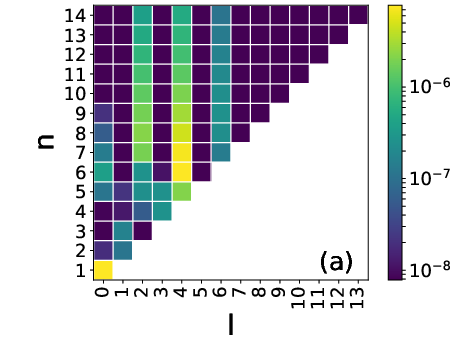
\includegraphics[width=0.32\columnwidth]{figs/Rydberg/heat_20_cyc_3p4e13_rev.png}
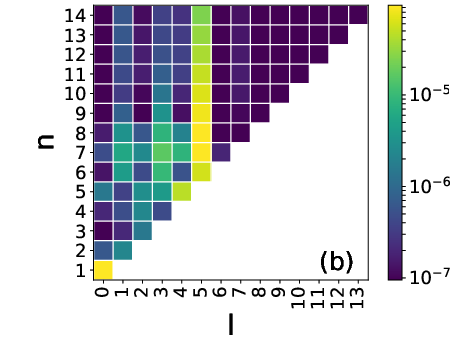
\includegraphics[width=0.32\columnwidth]{figs/Rydberg/heat_20_cyc_6p0e13_rev.png}\\
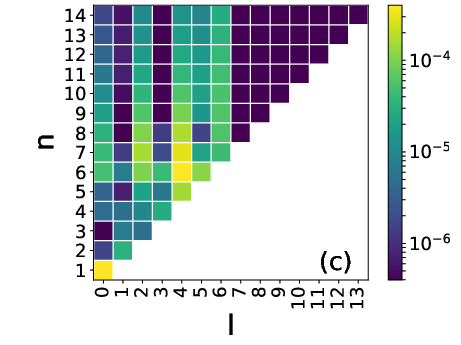
\includegraphics[width=0.32\columnwidth]{figs/Rydberg/heat_20_cyc_8p6e13_rev.png}
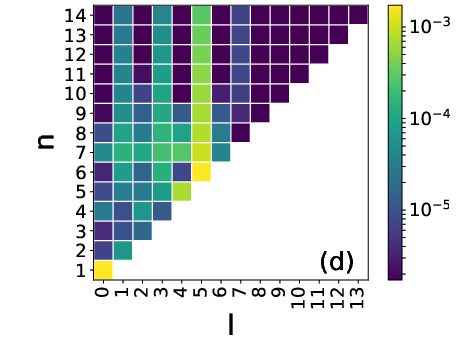
\includegraphics[width=0.32\columnwidth]{figs/Rydberg/heat_20_cyc_11p2e13_rev.png}
\caption{\label{fig:parity}
Excited state distribution as function of $n$ (vertical axis) and $l$ (horizontal axis) at the end of 20 cycle pulses with sine-squared envelope and peak intensities: 
(a) $I_0 = 3.4\times10^{13}$ W/cm$^2$, 
(b) $I_0 = 6.0\times10^{13}$ W/cm$^2$, 
(c) $I_0 = 8.6\times10^{13}$ W/cm$^2$, and 
(d) $I_0 = 1.12\times10^{14}$ W/cm$^2$. 
Left (right) column corresponds to cases in which the Rydberg states are resonant with an even (odd) number of photons. (Figure taken from \cite{venzke2018_ryd})
}
\end{figure}

\begin{figure}[!ht]
\centering
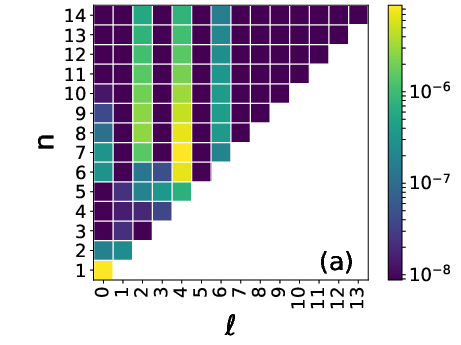
\includegraphics[width=0.32\columnwidth]{figs/Rydberg/heat_14_cyc_gauss_3p4e13.png}
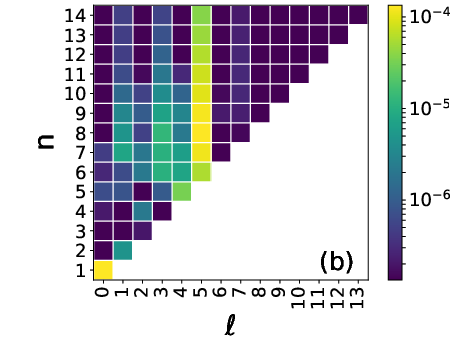
\includegraphics[width=0.32\columnwidth]{figs/Rydberg/heat_14_cyc_gauss_6p0e13.png}\\
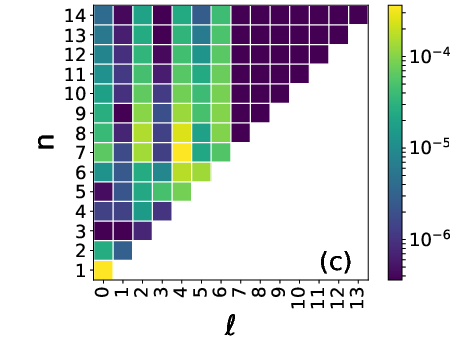
\includegraphics[width=0.32\columnwidth]{figs/Rydberg/heat_14_cyc_gauss_8p6e13.png}
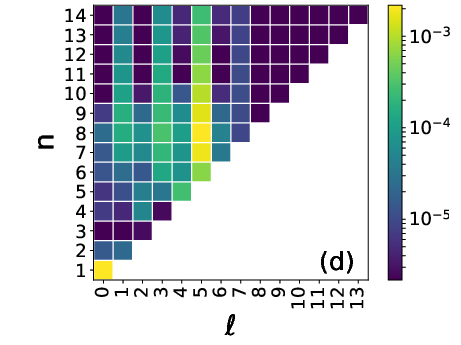
\includegraphics[width=0.32\columnwidth]{figs/Rydberg/heat_14_cyc_gauss_11p2e13.png}
\caption{\label{fig:parity_gauss}
Same as Fig.~\ref{fig:parity} but for pulses with Gaussian envelope and 14 cycles FWHM. The pulse duration approximately matches that for the sine-squared pulses in Fig.~\ref{fig:parity} at FWHM. (Figure taken from \cite{venzke2018_ryd})
}
\end{figure}

The population in each quantum state $(n, l)$ at the end of the pulse is shown in Fig.~\ref{fig:parity} (20 cycle pulses with sine-squared envelope) and Fig.~\ref{fig:parity_gauss} (14 FWHM cycle pulses with Gaussian envelope) for intensities between $10^{13}$ and $10^{14}$ W/cm$^2$. The results shown in the left (right) column correspond to cases in which the Rydberg states are resonant with an even (odd) number of photons. In all cases we see that the highest angular momentum states ($l>7$) are not vary populated, in agreement with previous studies \cite{piraux2017} and semiclassical estimates \cite{arbo2008}. In the results we indeed observe signatures of the selection rules resulting in dominant population of states with an even (odd) angular momentum quantum number for the absorption of even (odd) photons in the plots on the left (right). This shows that in the intensity regime of $10^{13}$ to $10^{14}$ W/cm$^2$ the parity selection rules, previously studied for monochromatic fields and flat-top pulses, are effective for long pulses of about 20 cycles. Since the parity effect is found to occur independent of the form of the envelope we restrict ourselves below to pulses with sine-squared envelope. However, we observe that the contrast between the population in even and odd states is stronger at lower intensities. We will further discuss this aspect in subsection \ref{ssub:pulse-length}.  

The results also show that for an odd parity process (right column) predominantly one angular momentum state ($l=5$) is populated. This is in agreement with the results presented by Li et al.\ \cite{li2014b}, who conjectured that electrons in the low angular momentum states more easily absorb additional photons resulting in suppression of population in these states due to ionization. However, our results for even parity processes exhibit a pattern, alternating in $l$, showing that both low and high angular momentum states, except for the $s$-states, remain populated at the end of the pulse. 

\begin{figure}[!ht]
\centering
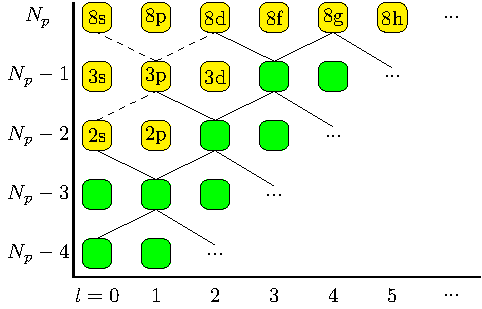
\includegraphics[width=0.49\columnwidth]{figs/Rydberg/l_fig_even.pdf}
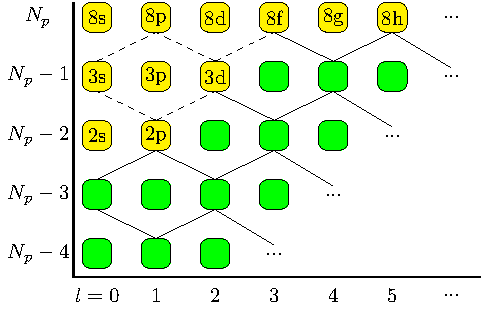
\includegraphics[width=0.49\columnwidth]{figs/Rydberg/l_fig_odd.pdf}
\caption{
The absorption pathways in an even (odd) photon process in the left (right) panel. Green squares represent virtual states with energy $N\omega$ above the ground state and angular momentum $l$. The yellow squares represent real states labeled by the quantum numbers. Solid lines refer to open pathways while dashed lines represent pathways which are suppressed due to population trapping in a lower excited state. (Figure taken from \cite{venzke2018_ryd})
}
\label{fig:pathways_ryd_linear}
\end{figure}

We therefore put forward an alternative explanation. To this end, in Fig.\ \ref{fig:pathways_ryd_linear} we show the various pathways leading to a resonant population in the $n=8$ (and the other Rydberg) states for absorption of an even (top panel) or an odd (bottom panel) number of photons, termed by $N_p$. Starting from the $1s$ ground state, the absorption of successive photons proceeds through virtual states (depicted via empty green squares in Fig.\ \ref{fig:pathways_ryd_linear}), following the selection rule $\Delta l = \pm 1$. As mentioned above, for the hydrogen atom and a pulse at a central wavelength of 800 nm the (shifted) $n=3$ and $n=2$ states are approximately resonant via $N_p-1$ and $N_p-2$ photon processes, as shown in Fig.\ \ref{fig:pathways_ryd_linear} (real states are depicted by yellow squares labeled with quantum number $nl$). Assuming that the resonant transitions to lower lying energy levels cause a trapping of population in these states, further absorption from these states will be suppressed. Such suppressed pathways are denoted by dashed lines in Fig.\ \ref{fig:pathways_ryd_linear}, while other (open) pathways are represented by solid lines. Following the pathways, we see that in the manifold of the Rydberg levels for an even number photon process (left panel) the $l = 2$ state is partially and the $l = 4, 6, \ldots$ states are fully accessible, while the $l=0$ ($s$-state) should be suppressed, which is in agreement with the pattern, alternating in $l$, that we observe in Figs.\ \ref{fig:parity} and \ref{fig:parity_gauss} (left columns). In contrast, for an odd number photon process (right panel) the pathways to the $l=1$ states are strongly and those to the $l=3$ states are partially suppressed, making the states with $l=5$ state the first fully accessible states among the Rydberg levels, in agreement with the results presented in Figs.\ \ref{fig:parity} and \ref{fig:parity_gauss} (right columns).

\subsubsection{Short vs. long pulses and CEP effects}
\label{ssub:pulse-length}

\begin{figure}[!ht]
\centering
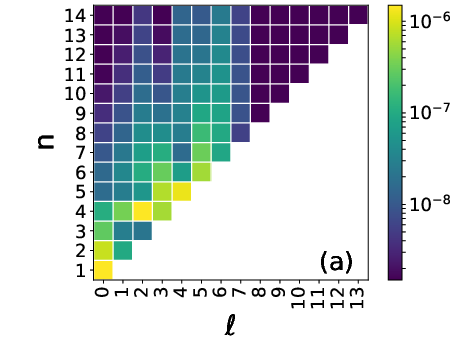
\includegraphics[width=0.32\columnwidth]{figs/Rydberg/heat_02_cyc_3p4e13.png}
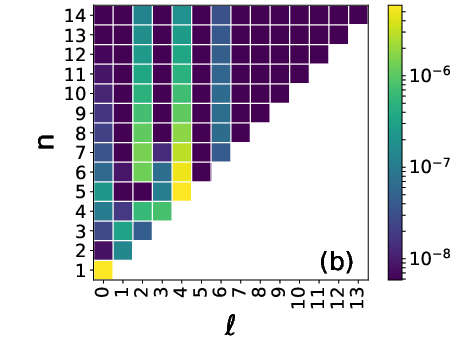
\includegraphics[width=0.32\columnwidth]{figs/Rydberg/heat_10_cyc_3p4e13.png}
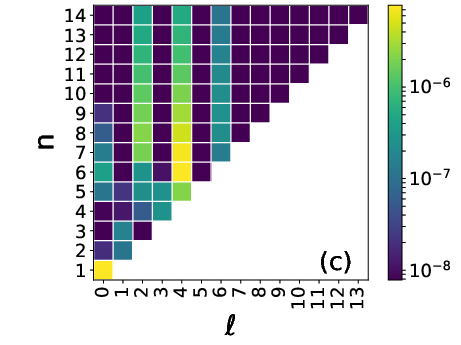
\includegraphics[width=0.32\columnwidth]{figs/Rydberg/heat_20_cyc_3p4e13_c.png}
\\
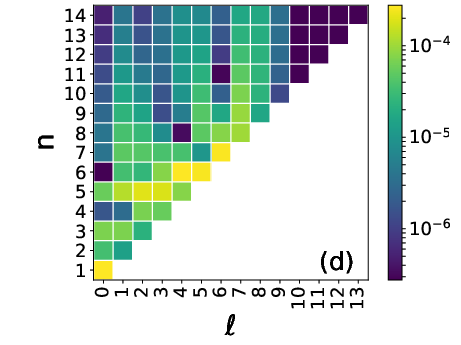
\includegraphics[width=0.32\columnwidth]{figs/Rydberg/heat_02_cyc_16p4e13.png}
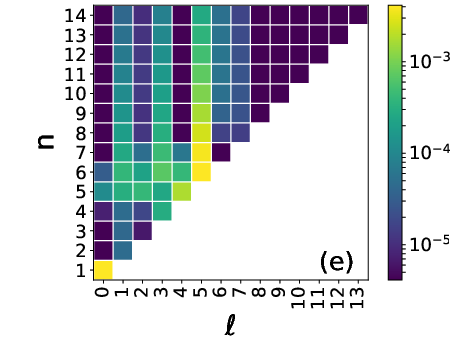
\includegraphics[width=0.32\columnwidth]{figs/Rydberg/heat_10_cyc_16p4e13.png}
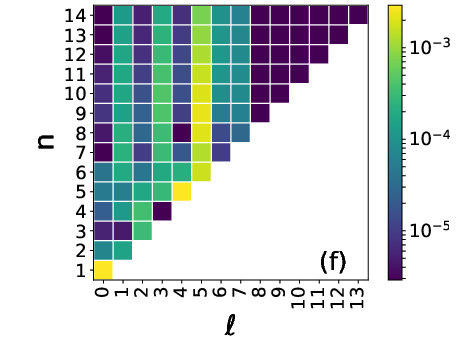
\includegraphics[width=0.32\columnwidth]{figs/Rydberg/heat_20_cyc_16p4e13.png}
\caption{\label{fig:length}
Excited state distribution as function of $l$ (horizontal axis) and $n$ (vertical axis) at the end of 2 cycle (panels on left), 10 cycle (panels in middle), and 20 cycle (panels on right) pulses, at low peak intensity $I_0 = 3.4 \times 10^{13}$ W/cm$^2$ (top row), and high peak intensity $I_0 = 1.64 \times 10^{14}$ W/cm$^2$ (bottow row). (Figure taken from \cite{venzke2018_ryd})
}
\end{figure}

The time-frequency uncertainty relation yields that a pulse spectrum broadens as the number of optical cycles decreases. Consequently, in an ultrashort pulse an excited state can be reached via absorption of different number of photons. Due to this mix of even and odd number of photon processes one may expect that in such pulses a separation in population of odd vs. even angular momentum quantum states cannot be achieved. This is confirmed by the results of our numerical calculations at low and high intensities, shown in Fig.~\ref{fig:length}(a) and (d). For a 2 cycle pulse there is a smooth distribution over the lower angular momentum states for each principal quantum number at low ($3.4 \times 10^{13}$ W/cm$^2$, panel (a)) and high ($1.64 \times 10^{14}$ W/cm$^2$, panel (d)) peak intensity.   

In contrast, the narrowing of the energy spectrum as pulse duration increases does not necessarily lead to an increase of the population in the angular momentum states of one parity over the other. For the low intensity 10-photon resonant process ($3.4 \times 10^{13}$ W/cm$^2$, Fig.\ \ref{fig:length}, upper row) we observe in the numerical results that Rydberg states with a well defined angular momentum parity are predominantly populated when the pulse duration is increased to 10 and 20 cycles. On the other hand, at the higher intensity ($1.64 \times 10^{14}$ W/cm$^2$, Fig.\ \ref{fig:length}, lower row) we observe some contrast between the population in the angular momentum states of different parity for the 10 cycle pulse (panel (e)), while the differences in the population of the different channels further blurs when the duration is increased to 20 cycles (panel (f)). 

Within the interpretation of resonant excitation the loss of the parity effect for long pulses with high peak intensities can be understood as follows. At the higher peak intensity, the highly excited states are shifted into resonance for 10-14 photon processes over the rising and trailing parts of the pulse, before they are resonantly excited with a 15 photon process at the peak intensity. Although the excitation probability raises with an increase of the intensity during the pulse, the time intervals over which the states are in resonance with a certain photon-order process increase with the pulse length. Thus, there is a significant excitation of the Rydberg states due to the absorption of odd as well as even numbers of photons in a pulse at high peak intensity and long duration. 

\begin{figure}[!ht]
\centering
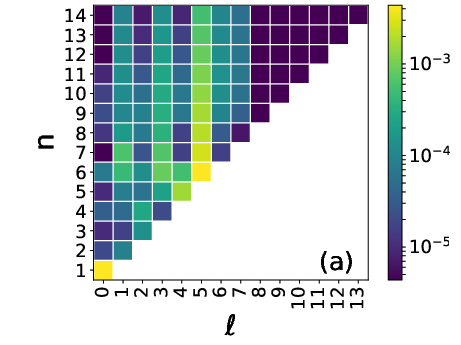
\includegraphics[width=0.32\columnwidth]{figs/Rydberg/heat_cep_test_0p102_20_cyc_16p4e13.png}
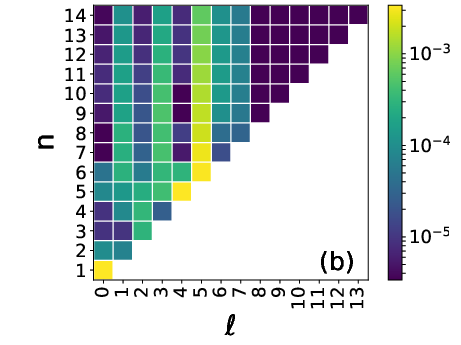
\includegraphics[width=0.32\columnwidth]{figs/Rydberg/heat_cep_test_0p441_20_cyc_16p4e13.png}
\caption{\label{fig:CEP_Effects_20_cyc}
Population of excited states from a 20 cycle pulse with peak intensity of $I_0 = 1.64 \times 10^{14}$ W/cm$^2$ and CEP of $\phi_A=0.204\pi$ (a) and $\phi_A=0.882\pi$ (b). (Figure taken from \cite{venzke2018_ryd})}
\end{figure}

Furthermore, excitation channels driven by absorption of different numbers of photons with the same parity may interfere, leading to the enhancement or suppression of population in certain angular momentum states and the loss of the parity effect. Interference effects in excitation have been studied extensively in the few-photon regime. Among others, it has been shown that the excitation probabilities can be controlled via the carrier envelope phase (CEP) of the pulse, even in the long pulse limit (e.g., \cite{zhao2013,zhao2014}). We observe in the results presented in Fig.\ \ref{fig:CEP_Effects_20_cyc} that the population distribution in the angular momentum states driven by the present more complex multiphoton processes indeed changes significantly with variation of the CEP at high intensities, indicative of potential interference effects.

We note that there may exist alternative explanations for the loss of the parity effect in the distribution at long pulses with high peak intensity. For example, in the tunneling regime the mechanism of frustrated ionization has been explored \cite{nubbemeyer2008}. According to that mechanism highly excited states are populated during the trailing edge of the pulse by deceleration of the electron over many laser cycles and electron recapturing once the laser pulse ceases. Since excited states of any angular momentum can be populated during the recapturing, the loss of the parity effect for long pulses at intensities in the tunneling regime is consistent with the frustrated ionization mechanism as well.

\subsection{Radiation spectra}
\label{sub:radiation}

It has recently been discussed \cite{chini2014,camp2015,beaulieu2016} that the population of excited Rydberg states leads to the emission of radiation due to the transition from the excited states into the ground state, which can be observed in the below-threshold part of high harmonic spectra. In the case of atomic hydrogen such emission is associated with an excitation of the $np$ states. In view of the parity effect in the excitation of the Rydberg states according to the absorption of an even or odd number of photons, we expect that the emission may be enhanced or suppressed in certain intensity regimes. To allow for the separation between the field induced and field free radiation we have calculated the high harmonic spectrum from the dipole acceleration $a(t)$ such that
%
\begin{equation}
f_{HHG}(\omega; t_f)  \propto \int\limits_{-\infty}^{t_f}  a(t') e^{-i\omega t'} dt'.
\end{equation}

\begin{figure}[!ht]
\centering
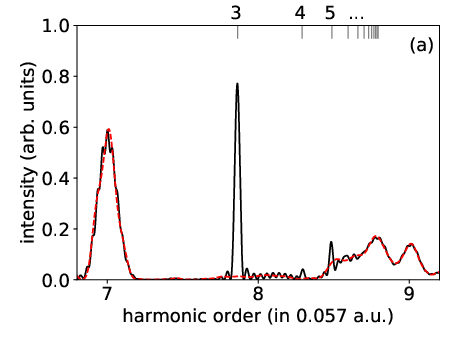
\includegraphics[width=0.32\columnwidth]{figs/Rydberg/HHG_3p4e13.png}
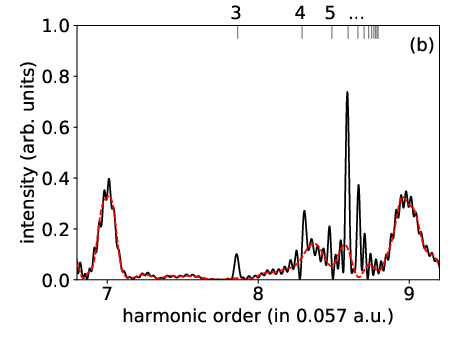
\includegraphics[width=0.32\columnwidth]{figs/Rydberg/HHG_6p0e13.png}
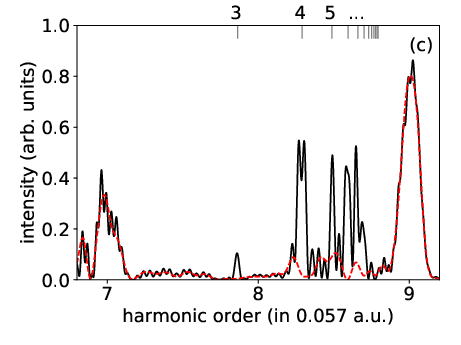
\includegraphics[width=0.32\columnwidth]{figs/Rydberg/HHG_16p4e13.png}
\caption{Radiation spectra generated during the pulse (red dashed lines) and those including line emissions after the pulse (black solid lines) are shown for peak intensities:
(a) $I_0 = 3.4\times10^{13}$ W/cm$^2$, 
(b) $I_0 = 6.0\times10^{13}$ W/cm$^2$, and
(c) $I_0 = 1.64\times10^{14}$ W/cm$^2$.
The vertical gray lines show the field free energy differences between the $np$ energy levels (up to $14p$) and the $1s$ ground state. (Figure taken from \cite{venzke2018_ryd})
}
\label{fig:HHG_6_10}
\end{figure}

In Fig.~\ref{fig:HHG_6_10} we present the radiation spectrum in the region of the 7th and 9th harmonics produced by a 20 cycle, sin squared, 800 nm pulse at intensities (a) $I_0 = 3.4\times10^{13}$ W/cm$^2$, (b) $I_0 = 6.0\times10^{13}$ W/cm$^2$, and (c) $I_0 = 1.64\times10^{14}$ W/cm$^2$. In each panel the red dashed line shows the spectrum generated during the pulse $(t_f = \tau)$ while the black solid line includes free propagation after the pulse has ended $(t_f = 2\tau)$. The difference between the two spectra exhibits the radiation related to the transitions from the populated excited $np$ states at the end of the pulse to the ground state, which has previously been identified in both experiment \cite{chini2014} and macroscopic simulations \cite{camp2015,beaulieu2016}.

Comparison of the spectra obtained at the two intensities clearly exhibits the expected difference in the features related to the parity effect in the population of the Rydberg states. At an intensity of $3.4\times10^{13}$ W/cm$^2$ (Fig.~\ref{fig:HHG_6_10}a), the (shifted) Rydberg energy levels are resonantly excited with a 10 photon process leading to population of the even angular momentum states. Consequently, the spectrum is free of line emission from the almost unpopulated Rydberg $p$-states while we find a strong line corresponding to the strongly populated $3p$ state, which is near resonant with a 9 photon process. In contrast, by shifting the states by the energy of an additional photon, at an intensity of $6.0\times10^{13}$ W/cm$^2$ (Fig.~\ref{fig:HHG_6_10}(b)) we observe a rich line emission spectrum just below the 9th harmonic line emissions from the $np$-states, that are resonantly populated by a 11 photon process. We note that the $6p$ and $7p$ states are the most populated $np$ states and as a result have the strongest emission lines. On the other hand the line corresponding to the $3p$ state, which cannot be populated by absorption of 10 photons, is strongly suppressed.

As discussed in section \ref{ssub:pulse-length}, at the highest intensity $I_0=1.64\times10^{14}$ W/cm$^2$, the population distribution in the angular momentum well defined parity begins to blur. This leads to a relatively even population in states with principle quantum number 4 to 14 seen in (Fig.~\ref{fig:length}(f)). As a result, we see in Fig.~\ref{fig:HHG_6_10}(c) line emission from all populated $np$ states with similar strengths for the states resolved in our spectrum.

\subsection{Summary}
\label{sub:summary}

We have analyzed in this section the angular momentum distribution in the Rydberg states of a hydrogen atom excited by a short strong laser pulse, based on numerical results of the time dependent Schr\"odinger equation, which we solved using a second order Crank-Nicolson scheme. At low intensities the pattern in the population across the angular momentum states can be explained via a parity effect due to the selection rules in multiphoton absorption along with the suppression of pathways due to population trapping in low excited states, if the applied laser pulse is not too short. At high intensities the parity effect gets lost even for long pulses, potentially since the Rydberg states are in resonance with photon processes of different orders for a significant time during the rising and trailing parts of the pulse. We predict that the parity effect can be observed via the strengths of the line emissions from the $np$ states emitted after the end of the pulse. 
% section linear_polarization (end)

%%%%%%%%%%%%%%%%%%%%%%%%%%%%%%%%%%%%%%%%%%%%%%%%%%%%%%%%%%%%%%%%%%%%%%%%%%%%%%%%%%%%%%%%%%%%%%%%%%%%%%%%%%%%%%%%%%
%%%%%%%%%%%%%%%%%%%%%%%%%%%%%%%%%%%%%%%%%%%%%%%%%%%%%%%%%%%%%%%%%%%%%%%%%%%%%%%%%%%%%%%%%%%%%%%%%%%%%%%%%%%%%%%%%%
%%%%%%%%%%%%%%%%%%%%%%%%%%%%%%%%%%%%%%%%%%%%%%%%%%%%%%%%%%%%%%%%%%%%%%%%%%%%%%%%%%%%%%%%%%%%%%%%%%%%%%%%%%%%%%%%%%
%%%%%%%%%%%%%%%%%%%%%%%%%%%%%%%%%%%%%%%%%%%%%%%%%%%%%%%%%%%%%%%%%%%%%%%%%%%%%%%%%%%%%%%%%%%%%%%%%%%%%%%%%%%%%%%%%%
%%%%%%%%%%%%%%%%%%%%%%%%%%%%%%%%%%%%%%%%%%%%%%%%%%%%%%%%%%%%%%%%%%%%%%%%%%%%%%%%%%%%%%%%%%%%%%%%%%%%%%%%%%%%%%%%%%
\section[Bi-circular polarization]{Bi-circular polarization\protect\footnote{The content of this section has been also published in J. Venzke, Y. Gebre, et al., Phys. Rev. A \textbf{101}, 053425  (2020).}} % (fold)
\label{sec:bi_circular_polarization}

% Recently, studies on th\textbf{e interaction of atoms and molecules with intense fields generated by the superposition of two circularly polarized laser pulses have seen an upsurge in activity in strong-field experiment and theory. For the most part, the renewed interest results from the capability to control the polarization of emitted light in high-order harmonic generation with such pulses. The physical principle has been proposed and applied first two decades ago 
% \cite{eichmann1995,long1995}. 
% More recently, efficient phase matching of circularly polarized high-order harmonic beams in the EUV and soft X-ray regime using bichromatic beams with counter-rotating circular polarization has been demonstrated \cite{fleischer2014,pisanty2014,kfir2015,fan2015,hickstein2015}. Since then, much experimental and theoretical work on high-harmonic generation \cite{milosevic2015a,medisauskas2015,milosevic2015b,chen2016,baykusheva2016,hernandez2016,liu2016,mauger2016,bandrauk2016,reich2016b,odzak2016,dorney2017,fleischer2017,zhavoronkov2017,pisanty2017,baykusheva2017,lerner2017,ayuso2018,dixit2018,barreau2018,huang2018,jimenez2018,heslar2018,paufler2018,li2019}, 
% ionization and photoelectron momentum distributions
% \cite{ngoko2015,yuan2016,milosevic2016c,mancuso2016,milosevic2016b,mancuso2017,pengel2017,busuladzic2017,hoang2017,lin2017,abusamha2018,busuladzic2018,eckart2018,li2018,han2018,eckart2018b,liu2018,eicke2019,ge2019,kerbstadt2019,abusamha2019}, double ionization 
% \cite{mancuso2016b,eckart2016,ben2017,ngoko2017,yu2018,huang2018b,ma2019}
% and other strong-field processes \cite{yuan2015,buica2018,guo2019} driven by bichromatic circularly polarized laser pulses has been performed. One interesting aspect in these kind of strong-field interactions is the control of ionization via the helicity of the applied bichromatic pulses \cite{milosevic2016c,mancuso2016,liu2018}. Such studies complement related work on the dependence of the ionization rate by one-color circularly pulse on the relative helicity between the pulse and the electron in the atomic orbital
% \cite{barth2011,kazansky2012,herath2012,barth2013,bauer2014,barth2014,ooi2014,hartung2016,douguet2016,watzel2016,wang2017,zhang2017,eckart2018c,liu2018b,trabert2018}.

% For bichromatic circularly polarized laser pulses it has been observed that the probability to ionize an atom is significantly enhanced if the two fields are counter-rotating as compared to co-rotating fields \cite{mancuso2016}. The experimental observations were interpreted as due to the increased density of excited states accessible for resonant enhanced multiphoton ionization in the case counter-rotating fields. Results of numerical solutions of the time-dependent Schr\"odinger equation in Ref.\ \cite{mancuso2016} did confirm a close relation between the ratios of total excitation and ionization probabilities for counter-rotating and co-rotating circularly polarized laser pulses. However, the results for excitation of the atom were not further resolved by distributions over the quantum numbers (principal, angular momentum, magnetic). Such analysis potentially can shed further light on the role of excited states in the pathways to ionization since excitation in a resonant multiphoton process should rely on the spin-angular momentum selection rules for the absorption of circularly polarized photons ($\Delta l = \pm 1$ and $\Delta m = \pm 1$).

% More generally, analysis of the role of strong-field excitation has recently experienced a renaissance 
% \cite{nubbemeyer2008,eichmann2013,chini2014,zimmermann2015} 
% following earlier work 
% \cite{freeman1987,perry1989,agostini1989}.
% Concerning the distribution in the excited states with respect to the quantum numbers studies for the interaction of atoms with linearly polarized pulses have been performed only. Theoretical studies have considered the distribution of the population as a function of the principal and/or the angular momentum quantum number \cite{krajewska2012,li2014,li2014b,xiong2017,piraux2017,venzke2018_ryd}. In applications of Floquet theory for a monochromatic laser field \cite{krajewska2012} and numerical calculations for laser pulses with  trapezoidal \cite{piraux2017} and Gaussian or $\sin$-squared envelopes \cite{venzke2018_ryd} it has been analyzed how the parity of the populated angular momentum states in such pulses relates to the selection rules for linearly polarized pulses. In view of the recent experimental observations discussed above, we extend these studies to interaction of atoms with bichromatic circularly polarized laser pulses. Such study provides the interesting opportunity to not only resolve the excited state distribution with respect to the principal or angular orbital momentum quantum number, but in particular to consider the role of the magnetic quantum number as well. For our studies we make use of results of numerical solutions of the time-dependent Schr\"odinger equation (TDSE) for the interaction of the hydrogen atom with intense bich}romatic circularly polarized laser pulses.

% The paper is organized as follows: In section \ref{sec:theory} we briefly summarize the standard methods used to solve the time-dependent Schr\"odinger equation for the interaction of hydrogen atom with bicircular laser pulses. The results of the numerical calculations are then presented and analyzed in section \ref{sec:results}, first for co-rotating and then for couter-rotating pulses. In section \ref{sec:summary} we summarize the insights gained into the excitation pathways in bircircular pulses. 


The time-dependent Schr\"odinger equation for the interaction of a electron in the potential of the hydrogen atom with a superposition of two circularly polarized intense laser pulses in dipole approximation and velocity gauge is given in Eq.~\ref{eq:SAE}\footnote{The corresponding numerical code has been developed by another graduate student (Y. Gebre). Results of that code have been tested well against results obtained using length gauge with the numerical program described in this thesis.}.
% (we use Hartree atomic units $e = m_e = \hbar =1$): 
% %
% \begin{equation}
% i\frac{\partial}{\partial t}\Psi(\mathbf{r},t) = \left[-\frac{\nabla^2}{2} - \frac{-i\mathbf{A}(t) \cdot \nabla}{c}  - \frac{1}{r} \right]\Psi(\mathbf{r},t).
% \end{equation}
%
% where ${\bf A}(t)$ is the vector potential of the two laser pulses. 
The wavefunction $\Psi$ is expanded in spherical harmonics up to $l_{max} = 45$ and  $m_{max} = 45$. The radius is discretized using fourth order finite difference method with a grid spacing of 0.1 a.u. and a maximum radius of 750 a.u.\ with exterior complex scaling on the outer 38 a.u. of the grid. The wavefunction is propagated in time using the Crank-Nicolson method with a time step of 0.05 a.u. The choice of gauge was based on the faster convergence of calculations in the velocity gauge for expansions of the wavefunction in spherical harmonics \cite{cormier1996,han2010}. 

The interaction with the bicircular laser pulse is implemented via the total vector potential as:
\begin{equation}
{\bf A}(t) = {\bf A}_{\omega}(t) + {\bf A}_{2\omega}(t)
\end{equation}
where
\begin{eqnarray}
{\bf A}_\Omega(t) &=& A_{0,\Omega} \sin^2\left(\frac{\pi t}{\tau_{\Omega}}\right)
    \nonumber
      \\
      && \times \left[ 
      \sin\left(\Omega t \right) {\hat{\bf x} + \epsilon_{\Omega}\cos\left(\Omega t \right)} {\hat{\bf y}} \right]
\end{eqnarray}
for $\Omega = \omega$ and $2\omega$, respectively. $A_{0,\Omega} = \frac{c\sqrt{I_\Omega}}{\Omega}$, $\tau_{\Omega} = \frac{2\pi N_{\Omega}}{\Omega}$, and $c$ is the speed of light, where $I_{\Omega}$ is the peak intensity and $N_{\Omega}$ denotes the number of cycles. $\epsilon_{\Omega} = \pm 1$ denotes the helicity of the fundamental and 2nd harmonic pulse, respectively. 

%and $\phi_{\Omega}$ is the carrier-to-envelope phase of the respective pulse

We have performed numerical calculations for the interaction of hydrogen atom with co- and counter-rotating bicircular pulses operating at the central wavelengths of 800 nm and 400 nm. Intensities of the two pulses were varied to study the distribution in the excited states as function of all quantum numbers, principal, angular momentum and magnetic. For the results presented below we have used pulses with the same pulse duration in time.  


% In this section we present the results for the distributions, first for the co-rotating and then for the counter-rotating case, which provide insights into selection rules and excitation pathways in bichromatic multiphoton processes.

\subsection{Excitation with co-rotating pulses}

\begin{figure}[!ht]
\centering
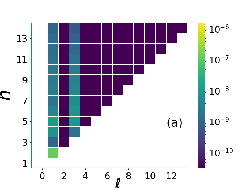
\includegraphics[width=0.24\columnwidth]{figs/Rydberg/Gebre-bicircular-Fig1a.png}
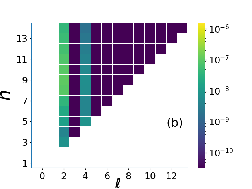
\includegraphics[width=0.24\columnwidth]{figs/Rydberg/Gebre-bicircular-Fig1b.png}
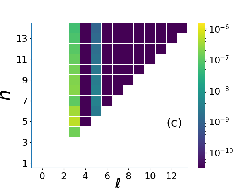
\includegraphics[width=0.24\columnwidth]{figs/Rydberg/Gebre-bicircular-Fig1c.png}
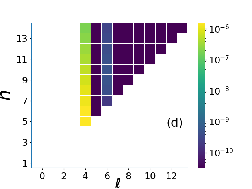
\includegraphics[width=0.24\columnwidth]{figs/Rydberg/Gebre-bicircular-Fig1d.png}
\caption{\label{fig:co-nl-distribution}
Excited state distribution as function of $n$ (vertical axis) and $\ell$ (horizontal axis) for (a) $m = -1$, (b) $m=-2$, (c) $m=-3$ and (d) $m=-4$ at the end of 20 (at 800 nm) cycle pulses (40 cycle at 400 nm) with sin squared envelope and total peak intensity of $1\times10^{14}$ W/cm$^2$ for co-rotating laser pulses of equal intensity. (Figure taken from \cite{venzke2020_ryd})
}
\end{figure}

Selection rules for (single-)photon absorption from circularly polarized light are given by $\Delta l = \pm 1$ and $\Delta m = \pm 1$, where the change in the magnetic quantum number is positive (negative) if the helicity of the light is right- (left-)handed. Extending the concept to multiphoton absorption, the simultaneous change in both quantum numbers puts distinct constraints on the parity and helicity of the accessible excited states in the atoms upon absorption of multiple photons. Specifically, it is expected that states in which $\ell$ and $m$ are either both even or both odd are being populated during the interaction with the field. This selection holds for the interaction with a single circularly polarized pulse as well as for the case of a superposition of two (or more) of such fields, independent of the relative helicity of the two pulses. 

In Fig.~\ref{fig:co-nl-distribution} we show examples of the population in the excited states of hydrogen atom as a function of $n$ and $\ell$ for various $m$ values at the end of the interaction with bichromatic co-rotating left-handed circularly polarized pulses. The results clearly confirm the expected population distribution in states with either odd or even parity for a given value of $m$ according to the selection rules upon multiphoton absorption. The present results have been obtained for interaction with equal peak intensities $I_{400} = I_{800} = 5\times 10^{13}$ W/cm$^2$. 

Due to the correlation in changes of $m$ and $\ell$ the observed pattern is independent of total peak intensity, ratio of peak intensities and pulse duration, as long as the dipole approximation holds. In our studies we have verified this up to intensities of $1 \times 10^{14}$ W/cm$^2$. This is different from the case of linear polarization \cite{venzke2018_ryd}, where selective population concerning the parity of the populated excited states is observed for long pulses and low peak intensities only. In that case the restriction to a given $m$-channel and a broad energy spectrum (for short pulse durations) or a significant Stark shift of the excited states (at high peak intensities) leads to a mixing of population over the states with odd and even orbital angular momentum quantum numbers.

\begin{figure}[!ht]
 \centering
  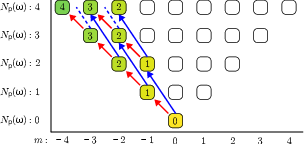
\includegraphics[width=0.75\columnwidth]{figs/Rydberg/co_rotating_absorbtion.png}
 \caption{\label{fig:co-pathways}
 Absorption pathways in co-rotating laser pulses at frequencies $\omega$ and $2 \omega$ starting from a $m=0$-state. Without lack of generalization it is assumed that both pulses have left-handed helicity. Absorption of a photon at frequency $\omega$ and at frequency $2 \omega$ is represented by a red and blue arrow, respectively. The numbers in the boxes denote the minimum number of photons to reach a certain level. (Figure taken from \cite{venzke2020_ryd})
 }
 \end{figure}

In co-rotating bicircular laser pulses all the photons have the same spin (either $+1$ or $-1$), consequently the magnetic quantum number always changes either by $\Delta m = +1$ or by $\Delta m = -1$ upon absorption of each photon. For our studies we have chosen left-handed helicity for both pulses and, hence, only excited states with negative $m$ can be populated upon absorption of photons from the ground state with $m=0$ (c.f., Fig.\ \ref{fig:co-pathways}). Therefore, as already mentioned in Ref.\ \cite{mancuso2017}, only Rydberg states with high orbital angular quantum number $\ell$ are accessible. For example, for excitation of Rydberg states (with $n \ge 4$) in the hydrogen atom, the absorption of at least 4 photons in laser field at 400 nm or at least 8 photons at 800 nm is required. Thus, Rydberg states with $\ell < 4$ (and $m > -4$) cannot be populated just via photon absorption alone.

\begin{figure}[!ht]
\centering
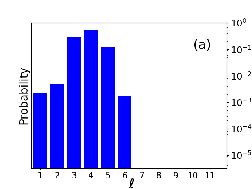
\includegraphics[width=0.24\columnwidth]{figs/Rydberg/Gebre-bicircular-Fig3a.png}
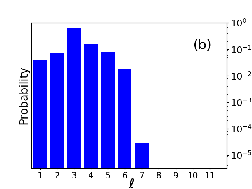
\includegraphics[width=0.24\columnwidth]{figs/Rydberg/Gebre-bicircular-Fig3b.png}
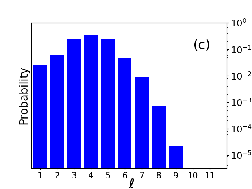
\includegraphics[width=0.24\columnwidth]{figs/Rydberg/Gebre-bicircular-Fig3c.png}
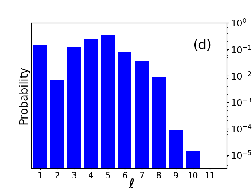
\includegraphics[width=0.24\columnwidth]{figs/Rydberg/Gebre-bicircular-Fig3d.png}
\caption{\label{fig:l-distribution}
Excited state distribution as function of orbital angular quantum number $\ell$ summed over $n \ge 4$ and $m$ at 
(a) $I_{400} = 5 \times 10^{13}$ W/cm$^2$, $I_{800} = 5 \times 10^{12}$ W/cm$^2$, 
(b) $I_{400} = 5 \times 10^{13}$ W/cm$^2$, $I_{800} = 1 \times 10^{13}$ W/cm$^2$, 
(c) $I_{400} = 5 \times 10^{13}$ W/cm$^2$, $I_{800} = 5 \times 10^{13}$ W/cm$^2$, and
and (d) $I_{400} = 1 \times 10^{13}$ W/cm$^2$, $I_{800} = 5 \times 10^{13}$ W/cm$^2$. Pulse durations: 20 cycles at 400 nm, 10 cycles at 800 nm. (Figure taken from \cite{venzke2020_ryd})
}
\end{figure}

Accordingly, the angular momentum distribution in the Rydberg states is controlled via the relative intensity of the two fields at the fundamental and second harmonic frequency. This is demonstrated in Fig. \ref{fig:l-distribution}, where the excited state distribution as a function of $\ell$, summed for $n \ge 4$ and all $m$, is shown. For large ratio of $I_{400}/I_{800} = 10$ (panel (a)) the distribution is centered, as expected, about $\ell = 4$. As the intensity ratio decreases, high orbital angular momentum states get increasingly populated due to the impact of the laser pulse at 800 nm. 

\begin{figure}[!ht]
\centering
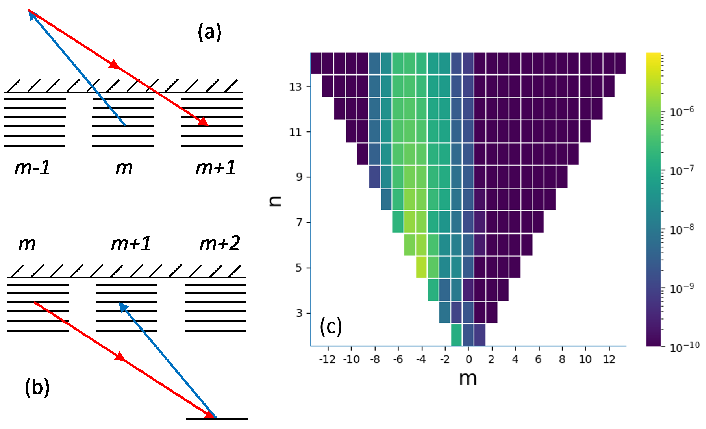
\includegraphics[width=0.6\columnwidth]{figs/Rydberg/Gebre-bicircular-Fig4.png}
\caption{\label{fig:nm-distribution}
Excited state distribution as function of $n$ (vertical axis) and $m$ (horizontal axis) summed over $\ell$. Laser parameters: 20 (800 nm) cycle pulses with sin squared envelope and total peak intensity of $1\times10^{14}$ W/cm$^2$ for co-rotating laser pulses of equal intensity. (Figure taken from \cite{venzke2020_ryd})
}
\end{figure}

Another interesting feature in Fig. \ref{fig:l-distribution} is that the population in angular momentum states with $\ell < 4$ increases significantly when the intensities of the two pulses are similar. Further insight can be gained by the distribution over the magnetic quantum number, which is displayed in Fig.~\ref{fig:nm-distribution}(c) for the case of equal intensities. It is clearly seen that Rydberg states with magnetic quantum numbers between $m=0$ and $m=-3$ are populated. In view of the number of photons needed to reach the Rydberg levels, the population in these states cannot be explained by absorption of photons only. 

Instead, we propose the following mechanism: Initially, Rydberg states with $\ell \ge 4$ are populated via the absorption pathways shown in Fig.\ \ref{fig:co-pathways}. Then a redistribution of population occurs via Raman-type $\Lambda$-transitions (c.f., \cite{gray1978,fedorov1996}). In the present bichromatic laser field the $\Lambda$-process leads to a change in the magnetic quantum number, if photons from both fields are involved. For the absorption of one 400 nm photon and emission of two 800 nm photons the magnetic quantum number between initial and final state changes by $\Delta m = +1$.
 
The order of absorption and emission may vary, i.e., the redistribution process can either proceed via the continuum (absorption first, Fig.~\ref{fig:nm-distribution}(a)) or via a lower excited state (emission first, Fig.~\ref{fig:nm-distribution}(b)). A larger change in $m$ is achieved either via a sequence of these $\Lambda$-processes or by higher order processes (e.g., absorption of two 400 nm photons followed by emission of four 800 nm photons leading to $\Delta m = +2$). We note that similarly the absorption of two photons at 800 nm and the emission of a 400 nm photon will lead to a change of $\Delta m = -1$ in the present set-up and, hence, contribute to population of states with higher $\ell$ and $m$.

\begin{figure}[!ht]
\centering
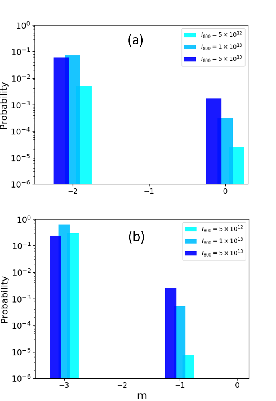
\includegraphics[width=0.5\columnwidth]{figs/Rydberg/Gebre-bicircular-Fig5.png}
\caption{\label{fig:nm-fixedl-distribution}
{
Distribution in magnetic quantum states for (a) $\ell = 2$ and (b) $\ell = 3 $ and different peak intensities of the 800 nm pulse. $I_{400} = 5\times 10^{13}$ W/cm$^2$ and other parameters are as in Fig.~\ref{fig:nm-distribution}. (Figure taken from \cite{venzke2020_ryd})}
}
\end{figure}

Our interpretation is further supported by the results in Fig.~\ref{fig:nm-fixedl-distribution}, which shows how the population in states of certain quantum numbers for (a) $\ell = 2$ and (b) $\ell = 3$ changes as function of the relative intensity of the two pulses. It is clearly seen that the population in these quantum states, which are not accessible via direct absorption of photons from the ground state, increases as the intensity of the pulse at 800 nm increases. Thus, these results provide further indications that the presence of the redistribution process depends on the impact of both pulses and its effectiveness increases with increase of the total intensity, in agreement with our interpretation of a $\Lambda$-type process. The redistribution of population in Rydberg states via higher-order Raman-like process induced by co-rotating bi-circular laser fields has been further studied in a project led by another graduate student \cite{gebre2021}.

\subsection{Excitation with counter-rotating pulses}

\begin{figure}[!ht]
\centering
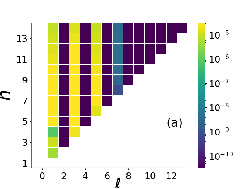
\includegraphics[width=0.24\columnwidth]{figs/Rydberg/Gebre-bicircular-Fig6a.png}
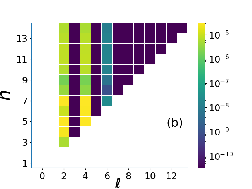
\includegraphics[width=0.24\columnwidth]{figs/Rydberg/Gebre-bicircular-Fig6b.png}
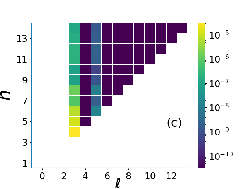
\includegraphics[width=0.24\columnwidth]{figs/Rydberg/Gebre-bicircular-Fig6c.png}
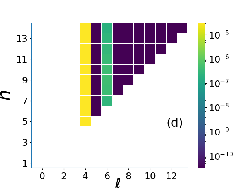
\includegraphics[width=0.24\columnwidth]{figs/Rydberg/Gebre-bicircular-Fig6d.png}
\caption{\label{fig:counter-nl-distribution}
Same as Fig.\ \ref{fig:co-nl-distribution} but for counterrotating laser pulses. (Figure taken from \cite{venzke2020_ryd})
}
\end{figure}

As discussed in the previous subsection, the selection rules by which only states with $\ell$ and $m$ either both even or both odd hold independent of the relative helicity of the two pulses. This is confirmed by the results that we obtained for the interaction with two counterrotating pulses at equal intensities and equal pulse duration presented in Fig.\ \ref{fig:counter-nl-distribution}. Depending on whether $m$ is even or odd, the distribution over the orbital angular momentum shows population in states with even or odd parity. As in the case of corotating pulses, the observed pattern is found independent of total peak intensity, ratio of peak intensities and pulse duration.


\begin{figure}[!ht]
 \centering
  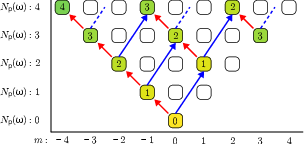
\includegraphics[width=0.75\columnwidth]{figs/Rydberg/counter_rotating_absorbtion.png}
 \caption{\label{fig:counter-pathways}
Absorption pathways in counter-rotating laser pulses at frequencies $\omega$ and $2 \omega$ starting from a $m=0$-state. Without lack of generalization it is assumed that the pulses at frequency $\omega$ has left-handed helicity, while the second harmonic pulse has right-handed velocity. Other symbols as in Fig. \ref{fig:co-pathways}. (Figure taken from \cite{venzke2020_ryd})
 }
 \end{figure}

Since in counter-rotating bicircular laser pulses photons of the two fields have opposite spin, starting from the ground state with $m=0$, excited states with both positive and negative magnetic quantum numbers can be populated. The absorption pathways for the set-up chosen in the present studies, namely right-handed helicity for the 800 nm pulse and left-handed helicity for the second harmonic, are shown in Fig.\ \ref{fig:counter-pathways}. As can be seen from the Figure, the magnetic quantum number reflects the difference between the number of 400 nm photons and that at 800 nm absorbed. Furthermore, it can be seen that for a given total photon energy absorbed states with magnetic quantum numbers separated by $\Delta m = \pm 3$ are populated. 

\begin{figure}[!ht]
\centering
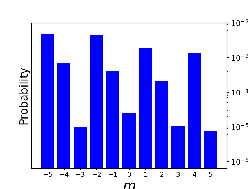
\includegraphics[width=0.49\columnwidth]{figs/Rydberg/Gebre-bicircular-Fig8a.png}
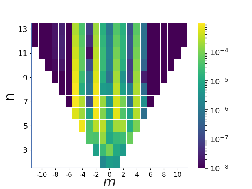
\includegraphics[width=0.49\columnwidth]{figs/Rydberg/Gebre-bicircular-Fig8b.png}
\caption{\label{fig:nm-counter-distribution}
Excited state distributions as a function of $m$, summed over $n \ge 4$ and $\ell$ (top), and as a function of $n$ and $m$, summed over $\ell$ (bottom), for the interaction with a left-handed circularly polarized laser pulse at 800 nm (20 cycles) and a right-handed circularly polarized laser pulse at 400 nm (40 cycles). Both pulses have the same peak intensity of $5 \times 10^{13}$ W/cm$^2$. (Figure taken from \cite{venzke2020_ryd})
}
\end{figure}

These features are clearly present in the population distributions as function of $m$, summed over $n$ and $\ell$ (top), and of $n$ and $m$, summed over $\ell$ (bottom), in Fig.\ \ref{fig:nm-counter-distribution}, which show the results for counter-rotating pulses of equal peak intensity. In the Rydberg manifold ($n \ge 4$) the highest populated $m$-states differ by $\Delta m = \pm 3$, other states show some but lower population as the manifold is AC-stark shifted during the interaction with the pulses. In view of the nonlinearity of multiphoton processes, it is likely that the states showing the largest probability are being populated near the peak of the pulses at which the highest total intensity is present. Overall, the strongest population is seen for states with negative magnetic quantum numbers, leading to the conclusion that it most likely that either five (for excited states with $m = -5$) or two (for excited states with $m = -2$) more 800 nm photons with left-handed helicity than 400 nm photons with right-handed helicity are being absorbed.    


\begin{figure}[!ht]
\centering
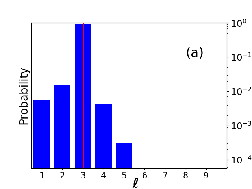
\includegraphics[width=0.32\columnwidth]{figs/Rydberg/Gebre-bicircular-Fig9a.png}
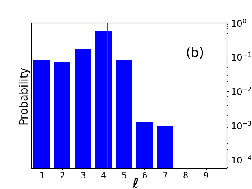
\includegraphics[width=0.32\columnwidth]{figs/Rydberg/Gebre-bicircular-Fig9b.png}
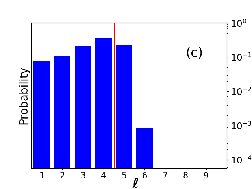
\includegraphics[width=0.32\columnwidth]{figs/Rydberg/Gebre-bicircular-Fig9c.png}
\caption{\label{fig:angular}
Orbital angular momentum distributions in excited states induced by counter-rotating laser pulses at 400 nm (20 cycles) and 800 nm (10 cycles) at peak intensities of (a) $I_{400} =  5 \times 10^{13}$ W/cm$^2$, $I_{800} = 5 \times 10^{12}$ W/cm$^2$, (b) $I_{400} = 5 \times 10^{12}$ W/cm$^2$, $I_{800} =  5 \times 10^{13}$ W/cm$^2$, and (c) $I_{400} = 5 \times 10^{13}$ W/cm$^2$, $I_{800} = 5 \times 10^{13}$ W/cm$^2$. (Figure taken from \cite{venzke2020_ryd})
}
\end{figure}

The distributions in Fig. \ref{fig:nm-counter-distribution} do not extend much beyond $|m| = 5$, which is consistent with the results shown in Fig. \ref{fig:angular} showing that there appears to be a highest orbital angular momentum number $\ell_{max}$ beyond which the population in the states drops off quickly. This is in agreement with previous studies for Rydberg state excitation \cite{piraux2017,venzke2018_ryd} and low energy angular momentum distributions \cite{arbo2008}. In Ref. \cite{arbo2008} a random walk analysis of the absorption pathways between the accessible quantum states is used to obtain the classical orbital angular momentum for a electron with zero energy in a laser field has been derived as $L = \sqrt{2Z\alpha_0}$
where $Z$ is the charge of the residual ion and $\alpha_0$ is the quiver radius. Relating classical orbital angular momentum and the orbital angular momentum quantum number by $\ell \approx L - 1/2$ we have estimated the maximum $\ell$ gained in the bicircular counter-rotating pulse. The estimates, shown by the solid red lines in Fig. \ref{fig:angular}, are in good agreement with the cut-offs seen in the numerical results. We note that the random walk analysis of Ref.\ \cite{arbo2008} can be applied in the case of counter-rotating pulses, since in each absorption step $\Delta m = \pm 1$ and hence, in general, $\Delta \ell = \pm 1$ is possible. In contrast, for co-rotating pulses the changes in magnetic and angular quantum number are determined in each absorption step ($\Delta m = -1$, $\Delta \ell = +1$) and hence a random walk analysis is not applicable and a cut-off cannot be derived.

\subsection{Summary}
\label{sub:summary_bi_circ_ryd}

In this section we have studied the distributions over the orbital angular momentum ($\ell$) and magnetic ($m$) quantum numbers in Rydberg states due to the interaction with bichromatic circularly polarized laser pulses. Multiphoton selection rules lead to population of states in which $\ell$ and $m$ are either both even or both odd, independent of relative helicity, peak intensity and pulse duration. In the case of co-rotating pulses the results show that the distribution over the magnetic quantum number can be controlled via the intensities of the two pulses. Furthermore, we propose that the states are populated via direct absorption from the ground state and via $\Lambda$-type transitions between Rydberg states of different $\ell$ and $m$, involving two photons at the fundamental wavelength and one photon at the second harmonic. For bicircular laser pulses with opposite helicities Rydberg states with magnetic quantum numbers that differ by $\Delta m = \pm 3$ are predominantly populated. The pattern allows to gain insights into the relative number of photons absorbed from the two fields. The distribution is however restricted by the maximum orbital angular momentum quantum number that can be estimated by classical considerations.
% section bi_circular_polarization (end)

% chapter rydberg_state_excitations (end)